% GNUPLOT: LaTeX picture with Postscript
\begingroup
  \makeatletter
  \providecommand\color[2][]{%
    \GenericError{(gnuplot) \space\space\space\@spaces}{%
      Package color not loaded in conjunction with
      terminal option `colourtext'%
    }{See the gnuplot documentation for explanation.%
    }{Either use 'blacktext' in gnuplot or load the package
      color.sty in LaTeX.}%
    \renewcommand\color[2][]{}%
  }%
  \providecommand\includegraphics[2][]{%
    \GenericError{(gnuplot) \space\space\space\@spaces}{%
      Package graphicx or graphics not loaded%
    }{See the gnuplot documentation for explanation.%
    }{The gnuplot epslatex terminal needs graphicx.sty or graphics.sty.}%
    \renewcommand\includegraphics[2][]{}%
  }%
  \providecommand\rotatebox[2]{#2}%
  \@ifundefined{ifGPcolor}{%
    \newif\ifGPcolor
    \GPcolortrue
  }{}%
  \@ifundefined{ifGPblacktext}{%
    \newif\ifGPblacktext
    \GPblacktexttrue
  }{}%
  % define a \g@addto@macro without @ in the name:
  \let\gplgaddtomacro\g@addto@macro
  % define empty templates for all commands taking text:
  \gdef\gplbacktext{}%
  \gdef\gplfronttext{}%
  \makeatother
  \ifGPblacktext
    % no textcolor at all
    \def\colorrgb#1{}%
    \def\colorgray#1{}%
  \else
    % gray or color?
    \ifGPcolor
      \def\colorrgb#1{\color[rgb]{#1}}%
      \def\colorgray#1{\color[gray]{#1}}%
      \expandafter\def\csname LTw\endcsname{\color{white}}%
      \expandafter\def\csname LTb\endcsname{\color{black}}%
      \expandafter\def\csname LTa\endcsname{\color{black}}%
      \expandafter\def\csname LT0\endcsname{\color[rgb]{1,0,0}}%
      \expandafter\def\csname LT1\endcsname{\color[rgb]{0,1,0}}%
      \expandafter\def\csname LT2\endcsname{\color[rgb]{0,0,1}}%
      \expandafter\def\csname LT3\endcsname{\color[rgb]{1,0,1}}%
      \expandafter\def\csname LT4\endcsname{\color[rgb]{0,1,1}}%
      \expandafter\def\csname LT5\endcsname{\color[rgb]{1,1,0}}%
      \expandafter\def\csname LT6\endcsname{\color[rgb]{0,0,0}}%
      \expandafter\def\csname LT7\endcsname{\color[rgb]{1,0.3,0}}%
      \expandafter\def\csname LT8\endcsname{\color[rgb]{0.5,0.5,0.5}}%
    \else
      % gray
      \def\colorrgb#1{\color{black}}%
      \def\colorgray#1{\color[gray]{#1}}%
      \expandafter\def\csname LTw\endcsname{\color{white}}%
      \expandafter\def\csname LTb\endcsname{\color{black}}%
      \expandafter\def\csname LTa\endcsname{\color{black}}%
      \expandafter\def\csname LT0\endcsname{\color{black}}%
      \expandafter\def\csname LT1\endcsname{\color{black}}%
      \expandafter\def\csname LT2\endcsname{\color{black}}%
      \expandafter\def\csname LT3\endcsname{\color{black}}%
      \expandafter\def\csname LT4\endcsname{\color{black}}%
      \expandafter\def\csname LT5\endcsname{\color{black}}%
      \expandafter\def\csname LT6\endcsname{\color{black}}%
      \expandafter\def\csname LT7\endcsname{\color{black}}%
      \expandafter\def\csname LT8\endcsname{\color{black}}%
    \fi
  \fi
  \setlength{\unitlength}{0.0500bp}%
  \begin{picture}(7200.00,5040.00)%
    \gplgaddtomacro\gplbacktext{%
      \csname LTb\endcsname%
      \put(1056,2520){\makebox(0,0)[r]{\strut{}$0.4$}}%
      \put(1056,3165){\makebox(0,0)[r]{\strut{}$0.5$}}%
      \put(1056,3809){\makebox(0,0)[r]{\strut{}$0.6$}}%
      \put(1056,4454){\makebox(0,0)[r]{\strut{}$0.7$}}%
      \put(1188,2300){\makebox(0,0){\strut{}}}%
      \put(1931,2300){\makebox(0,0){\strut{}}}%
      \put(2674,2300){\makebox(0,0){\strut{}}}%
      \put(3417,2300){\makebox(0,0){\strut{}}}%
      \put(4160,2300){\makebox(0,0){\strut{}}}%
      \put(4903,2300){\makebox(0,0){\strut{}}}%
      \put(5646,2300){\makebox(0,0){\strut{}}}%
      \put(6389,2300){\makebox(0,0){\strut{}}}%
      \put(418,3648){\rotatebox{-270}{\makebox(0,0){\strut{}$<\tilde{\phi}_{local}>$}}}%
      \put(6979,3648){\rotatebox{-270}{\makebox(0,0){\strut{}}}}%
      \put(3974,4666){\makebox(0,0){\strut{}}}%
      \put(3974,4665){\makebox(0,0){\strut{}}}%
      \put(264,2410){\makebox(0,0)[l]{\strut{}}}%
    }%
    \gplgaddtomacro\gplfronttext{%
      \put(5424,4603){\makebox(0,0){\strut{}Experiments}}%
      \csname LTb\endcsname%
      \put(5805,3569){\makebox(0,0)[r]{\strut{}$\phi=0.497$}}%
      \csname LTb\endcsname%
      \put(5805,3833){\makebox(0,0)[r]{\strut{}$\phi=0.535$}}%
      \csname LTb\endcsname%
      \put(5805,4097){\makebox(0,0)[r]{\strut{}$\phi=0.555$}}%
      \csname LTb\endcsname%
      \put(5805,4361){\makebox(0,0)[r]{\strut{}$\phi=0.576$}}%
    }%
    \gplgaddtomacro\gplbacktext{%
      \csname LTb\endcsname%
      \put(1056,704){\makebox(0,0)[r]{\strut{}$0.4$}}%
      \put(1056,1223){\makebox(0,0)[r]{\strut{}$0.5$}}%
      \put(1056,1741){\makebox(0,0)[r]{\strut{}$0.6$}}%
      \put(1056,2260){\makebox(0,0)[r]{\strut{}$0.7$}}%
      \put(1188,484){\makebox(0,0){\strut{}$0$}}%
      \put(1931,484){\makebox(0,0){\strut{}$0.1$}}%
      \put(2674,484){\makebox(0,0){\strut{}$0.2$}}%
      \put(3417,484){\makebox(0,0){\strut{}$0.3$}}%
      \put(4160,484){\makebox(0,0){\strut{}$0.4$}}%
      \put(4903,484){\makebox(0,0){\strut{}$0.5$}}%
      \put(5646,484){\makebox(0,0){\strut{}$0.6$}}%
      \put(6389,484){\makebox(0,0){\strut{}$0.7$}}%
      \put(418,1611){\rotatebox{-270}{\makebox(0,0){\strut{}$<\phi_{local}>$}}}%
      \put(6979,1611){\rotatebox{-270}{\makebox(0,0){\strut{}}}}%
      \put(3974,154){\makebox(0,0){\strut{}$Q_6$}}%
      \put(3974,2409){\makebox(0,0){\strut{}}}%
      \put(3974,2408){\makebox(0,0){\strut{}}}%
      \put(264,110){\makebox(0,0)[l]{\strut{}}}%
    }%
    \gplgaddtomacro\gplfronttext{%
      \put(5358,2346){\makebox(0,0){\strut{}Simulations}}%
      \csname LTb\endcsname%
      \put(5805,1048){\makebox(0,0)[r]{\strut{}$\phi=0.487$ }}%
      \csname LTb\endcsname%
      \put(5805,1312){\makebox(0,0)[r]{\strut{}$\phi=0.507$ }}%
      \csname LTb\endcsname%
      \put(5805,1576){\makebox(0,0)[r]{\strut{}$\phi=0.528$ }}%
      \csname LTb\endcsname%
      \put(5805,1840){\makebox(0,0)[r]{\strut{}$\phi=0.548$ }}%
      \csname LTb\endcsname%
      \put(5805,2104){\makebox(0,0)[r]{\strut{}$\phi=0.568$ }}%
    }%
    \gplbacktext
    \put(0,0){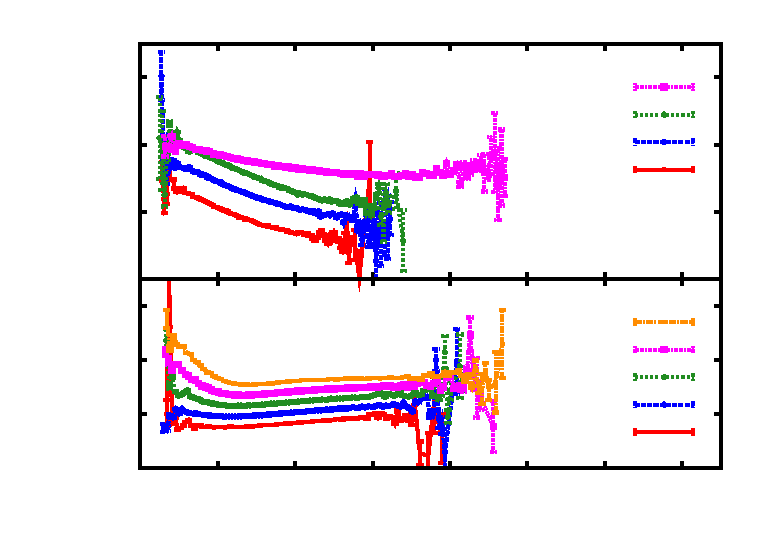
\includegraphics{phi_Q6_xpsim}}%
    \gplfronttext
  \end{picture}%
\endgroup
